\documentclass[a4paper,11pt,dvipdfmx]{ujarticle}
% パッケージ
\usepackage{graphicx}
\usepackage{url}
% レイアウト指定を記述したファイルの読み込み
\input{layout}

% タイトルと氏名を変更せよ.
\title{日本におけるデジタル化の状況}
\author{G584172025 安藤 駿}

\begin{document}

     
\maketitle %ここにタイトルが入る

% ここから本文
% 節見出し: \section{}
% を使う
\section{ブロードバンドの整備状況}


% 本文(1)
%  参考文献の参照: \cite{}
%  図番号の参照: \ref{}
% を使う
% 文献データベースのキーワードは oecd と imd
% になっている
OECDによるブローバンド回線の普及に関する\cite{OECD}によると、図\ref{hyou}に示すように、日本における
100人あたりのモバイルブローバンドの加入者は190.5で、第1位になっている。2位はエストニア
で、3位米国と続く。

% 図の挿入
% \includegraphics{}
% を
% \begin{figure}[htbp]
% \end{figure}
% で囲み
% \caption{}
% で図のタイトルを入れる.
% \label{}
% を使って図番号が参照できるようにする
% また,
% \centering
% で図が中央に来るようにする
\begin{figure}[htbp]
    \label{hyou}
    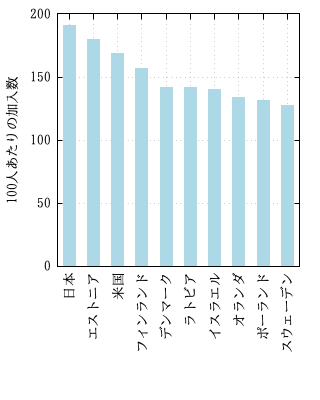
\includegraphics{fig21.png}
    \caption{光ファイバー回線の加入者(100人あたり)}
     \centering
\end{figure}


% ーーー
% 節見出し(2)
\section{デジタル競争力ランキング}

% 本文(2)
国際経営開発研究所(IMD)の調査\cite{IMD}によると、表\ref{tbl:利用状況}に示すように、日本のデジタル競争力ランキ
ングは調査対象の64カ国中、総合で28位、知識分野で25位になっている。

% 表の挿入
% \begin{tabular}
% \end{tabular}    
% による表の記述を 
% \begin{table}[htbp]
% \end{table}
% で囲み
% \caption{}
% で表のタイトルを入れる.
% \label{}
% を使って表番号が参照できるようにする
% また,
% \centering
% で表が中央に来るようにする
\begin{table}[htbp]
    \centering
    \caption{デジタル競争力ランキング(64カ国中)}
    \label{tbl:利用状況}

    \begin{tabular}{|c|r|r|}\hline
        国 & 総合 & 知識 \\
        \hline
        米国 & 1位 & 3位 \\
        \hline
        香港 & 2位 & 5位 \\
        \hline
        スウェーデン & 3位 & 2位 \\
        \hline
        デンマーク & 4位 & 8位 \\
        \hline
        シンガポール & 5位 & 4位 \\
        \hline
        \hline
        韓国 & 12位 & 15位 \\
        \hline
        中国 & 15位 & 6位 \\
        \hline
        \hline
        日本 & 28位 & 25位 \\
         \hline

        
        
    \end{tabular}
    
\end{table}

% ーーー
% 見出し(3)
\section{考察}

% 考察
%
% \begin{itemize}
% \end{itemize}
% を使って箇条書きで記述する
\begin{itemize}
    \item デジタル競争力ランキングは総合は28位で知識は25位となっており、デジタル化を推進するには、知識の強化が必要である
    \item ブローバンドの普及では上位だがデジタル競争力は遅れをとっているので日本の強みと弱みを明確にし、戦略的に取り組む必要がある
    \item インフラ整備をただするのではなく、デジタル技術を高めていくことも課題だと思う
\end{itemize}

% ここに参考文献が入る
%
\bibliographystyle{junsrt}
\bibliography{exercise.bib}

\end{document}